%%%%%%%%%%%%%%%%%%% author.tex %%%%%%%%%%%%%%%%%%%%%%%%%%%%%%%%%%%
%
% sample root file for your "contribution" to a contributed volume
%
% Use this file as a template for your own input.
%
%%%%%%%%%%%%%%%% Springer %%%%%%%%%%%%%%%%%%%%%%%%%%%%%%%%%%


% RECOMMENDED %%%%%%%%%%%%%%%%%%%%%%%%%%%%%%%%%%%%%%%%%%%%%%%%%%%
\documentclass[graybox]{svmult}

% choose options for [] as required from the list
% in the Reference Guide

\usepackage{mathptmx}       % selects Times Roman as basic font
\usepackage{helvet}         % selects Helvetica as sans-serif font
\usepackage{courier}        % selects Courier as typewriter font
\usepackage{type1cm}        % activate if the above 3 fonts are
                            % not available on your system
%
\usepackage{makeidx}         % allows index generation
\usepackage{graphicx}        % standard LaTeX graphics tool
                             % when including figure files
\usepackage{multicol}        % used for the two-column index
\usepackage[bottom]{footmisc}% places footnotes at page bottom
% see the list of further useful packages
% in the Reference Guide
\usepackage{longtable}
\usepackage[utf8]{inputenc}
\usepackage{array}
\makeindex             % used for the subject index
                       % please use the style svind.ist with
                       % your makeindex program

%%%%%%%%%%%%%%%%%%%%%%%%%%%%%%%%%%%%%%%%%%%%%%%%%%%%%%%%%%%%%%%%%%%%%%%%%%%%%%%%%%%%%%%%%
\newcolumntype{C}[1]{>{\centering\let\newline\\\arraybackslash}m{#1}}

\begin{document}

\title*{Predication Instances spot price in EC2}
\author{Sara Abdulaziz, Kyungyong Lee, and Hyeokman Kim}
\institute{Sara Abdulaziz \at Kookmin University, Seoul. South Korea, \email{name@email.address}
\and Kyungyong Lee \at Kookmin University, Seoul. South Korea, \email{leeky@kookmin.ac.kr}
\and Hyeokman Kim  \at Kookmin University, Seoul. South Korea, \email{hmkim@kookmin.ac.kr}
}
%
% Use the package "url.sty" to avoid
% problems with special characters
% used in your e-mail or web address
%
\maketitle

\abstract{We analyze G2 spot instance price}

\section{Introduction}\label{sec:1}
Cloud computing provides various types of compute resources to serve diverse application scenarios. The cloud computing frees the burden of system administration overheads without incurring prohibitive initial hardware purchase cost. From the service provider's perspective, fully utilizing the already established hardware resources and services is crucial to maximize monetary gain. As the users' resource demand can vary from time to time, some cloud computing providers offer services at chaper price than the regular price to maximize hardware/service utilization. For instance, Amazon Web Services (AWS), a leading cloud computing vendor, provides its surplus of EC2 computing resources at a cheaper price in the form of \emph{spot instance}. A user who wants to use spot instance bids for a price that one is willing to pay, and if the bid price is higher than the spot price that is decided by the service provider, one can get the resource allocated and pays for the spot price in the hourly basis. Other than AWS, Google Cloud Engine provides such opportunistic resources in the form of \emph{preemptive instances}, and Microsoft Azure provides its excess compute capacity as \emph{low-priority VM}.

Though users can utilize the opportunistic resources at a cheaper price, sudden service termination can happen at anytime as the demand for the computing resource changes. To mitigate the chance of sudden service interruption, few works were conducted to better predict and model the price change of EC2 spot instance in literature. Ben-Yehuda et al.~\cite{spot-instance-pricing-analysis} and Zhao et al.~\cite{spot-price-han-arima} tried to predict the future spot instance price using various predictive analysis algorithms, but they all concluded that the spot price is rather random and hard to make meaningful prediction for future price changes. Since then, most of studies that are related to the utilization of spot instance focus on the handling sudden service interruption~\cite{tr-spark,spot-mpi-checkpoint,flint,deep-spot-cloud} or spot instance bid strategy~\cite{not-bid-cloud,how-to-bid-cloud}. 

In this paper, we apply few time-series analysis algorithms to predict future price change pattern of AWS EC2 spot instances. By carefully desiging the period of train datasets, we could uncover that applying seasonal-arima (s-arima) can improve the accuracy of price change prediction error by 17\% on average comparing to the naive method that references most recent price to predict future price~\cite{deep-spot-cloud}. In addition to the contribution of improved price prediction accuracy, we could also discover that the configuration values to get the best prediction accuracy differs significantly across different availability zones (AZs) and instance types. Based on the extensive experiments and promising results, we bring up an opportunity of improving spot instance prediction accuracy that can result in significant cost gain for cloud computing users with increased system stability.


\section{Time-Series Analysis for AWS EC2 Spot Instance Price}
In our work, we use many forecasting time series models and parameters to get best fit to data, from sample models as mean method which use mean of history as predation, assume that our historical data sets be \(x\)
\begin{equation}
 \frac{y_t = x_{t-1} +x_{t-2}+ x_{t-3}+.....+x_{t-n}}{X}
\label{mean}
\end{equation} 

Naïve method another simple model to forecasting but anested to use mean historical data the model just simple set last value to be as predation result 
\begin{equation}
 y_t = x_{t-1} 
\label{naive}
\end{equation}
seasonal mean method to forecast time series the model use historical data to find the same \(S\) previous observed for predation at time T 
\begin{equation}
 y_t = x_s 
\label{smean}
\end{equation}

Where \(x\) previous observed from historical data at time \(s\) where \(s\) equal to \(t\)

ARIMA with different parameters 
stander for Autoregressive Integrated Moving Average, which is the most popular statistical model and widely used to forecasting a time series, the model is a combination of  autoregressive Eq.~\ref{Eq-AR} and moving-average model Eq.~\ref{Eq-MA}, with three parameters  \((p,d,q)\) where p is the number of autoregressive terms, which is depends on past values, d is the degree of differencing and  \(q\) is the number of lagged forecast errors in the prediction equation, depends only on the random error terms 
\begin{equation}
 y_t = w_0 +\beta_1 y_{t-1}+ \beta_2 y_{t-2}+.....\beta_n y_{t-n}+\epsilon_t
\label{Eq-AR}
\end{equation}
\begin{equation}
 y_t = w_0 +\epsilon_t + \delta_1 \epsilon_{t-1}+  \delta_2 \epsilon_{t-2}+...+ \delta_n \epsilon_{t-n}
\label{Eq-MA}
\end{equation}
Thus, ARIMA if \(d = n\) will be 
\begin{equation}
 y_t = w_0 +\beta_1 y_{t-1}+ \beta_2 y_{t-2}+.....\beta_n y_{t-n} +  \delta_1 \epsilon_{t-1}+  \delta_2 \epsilon_{t-2}+...+ \delta_n \epsilon_{t-n}+
\label{Eq-ARIMA}
\end{equation}
Where the term \(\beta_i \) is, weight applied to prior values in the time series \(\delta_i \) is autocorrelation coefficients at lags and \(\epsilon_i \) is residual error term 

\section{Evaluation}
To evalate the effectiveness of applying various algorithms to predict spot instance price, we fetch 11 months (March. 2016 ~ Feb. 2017) of spot price log files from the AWS public API service. From the log file, we extracted the timestamp, spot price, availability zone, and instance type. As the on-demand instance price is different for different instance types in different regions, we normalize the spot instance price to that of on-demand instance. The normailized value indicates the cost gain that one can expect while using spot instances.

At the time of writing, there are over 60s of AWS EC2 instance types that are served in over 30 availability zones. It becomes prohibitive to present the experiment results from all the instance types, and we select representative instances in General, GPU, Compute-, Memory-, and Storage-optimized types that are m4.2xlarge, g2.2xlarge, c3.2xlarge, r3.2xlarge, and i2.2xlarge, respectively. The instances are not served in all availability zones, and we choose 18 zones that provides the aformentioned instances types for experiments.

We evaluate naive, seasonal naive, mean, seasonal ARIMA, Linear Regression, and Prophet~\cite{prophet} algorithms using packages in R 3.2.4. Among them, Linear Regression and Prophet always perform worse than Arima, and we do not show the result. Different algorithms have distinct heuristic to choose the train dataset window. Naive and seasonal naive simply reference values from the previous observations. For mean method, we use previous 1, 3, 7, 15, 30, 60, 90, and 120 days to get mean value for prediction. However, using only the most recent data (1 day) shows the best result, and we exclude other results. For seasonal Arima, we differentiate the training dataset period as 30, 60, 90, 120, and 150 days. In the prediction step, we use a model built by \textit{auto.arima} method of R. After building a model, we use the model for the next 1, 4, 8, 15, and 30 days. Overall, seasonal Arima has two configurations in the modeling data, \emph{previous days used in modeling, the number of days for a model to be used}, and we notate the value using parenthesis. For all algorithms, we predict the normalized spot instance price for the next 24 hours and calculate root-mean-squared-error to evaluate each model.   

\begin{figure}
\centering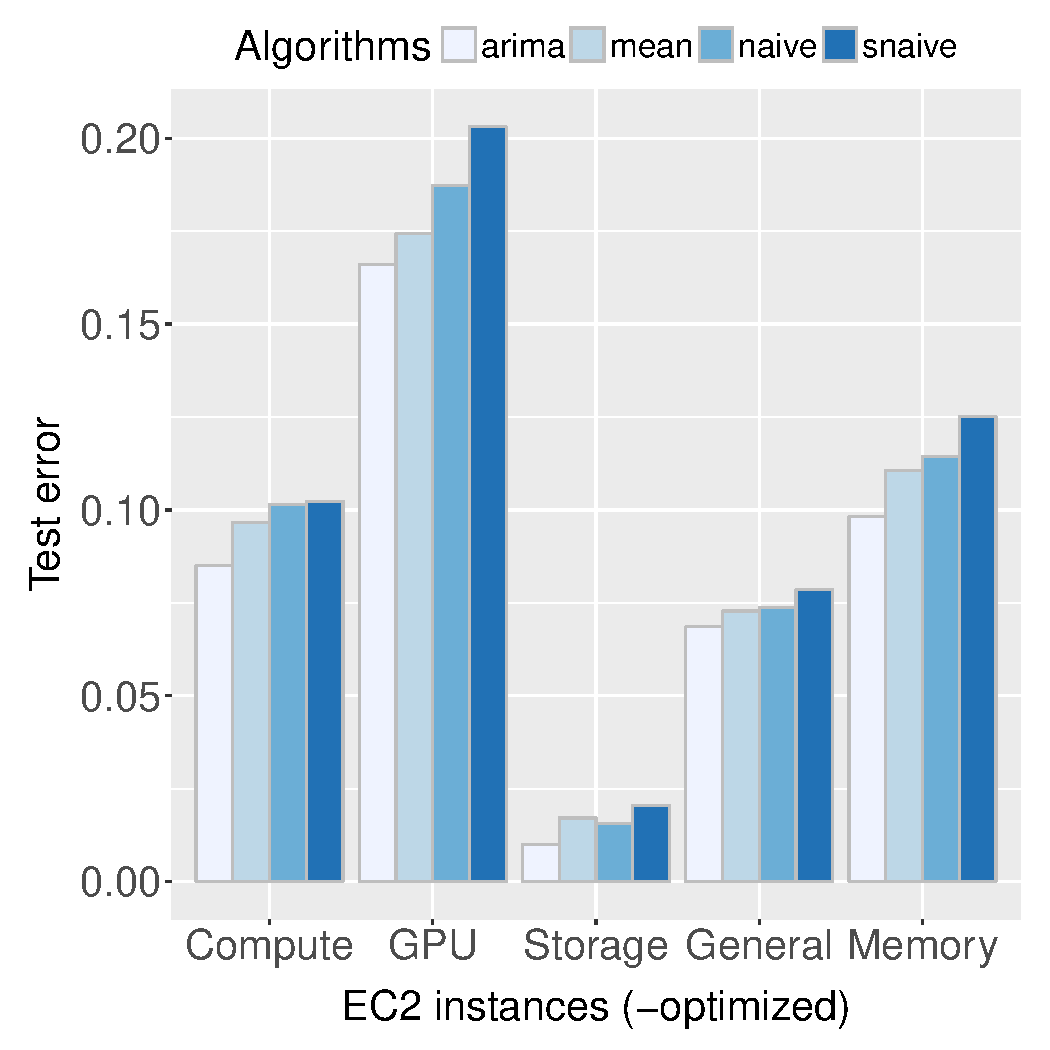
\includegraphics[width=0.7\textwidth]{figures/algorithm-compare-different-instance-type.pdf}\caption{Test error rates of different predictive algorithms. Regardless of the instance types, Arima shows the least error rate\label{fig:algo-diff-inst}}
\end{figure}
Figure~\ref{fig:algo-diff-inst} shows the test error of different algorithms. For seasonal Arima and mean, we select the best performing configuration values. Each algorithm is executed in all 18 availability zones, and the mean test error is presented. Regardless of instance types, Arima algorithm shows the best prediction accuracy among other methods. Previous studies concluded that using predictive analysis algorithms did not help to improve the prediction accuracy of spot instance price, and most system should rely only on the very recent price (naive method). However, with thorough experiments and train data modeling, we could uncover the effectiveness of using Arima model to predict spot instance price for the first time. In the figure, we can observe that different instance types show different test error rate, and we expect the different hardware specifications, such as equip with GPU card, can result in distinct supply and demand amounts.  

\begin{figure}
\centering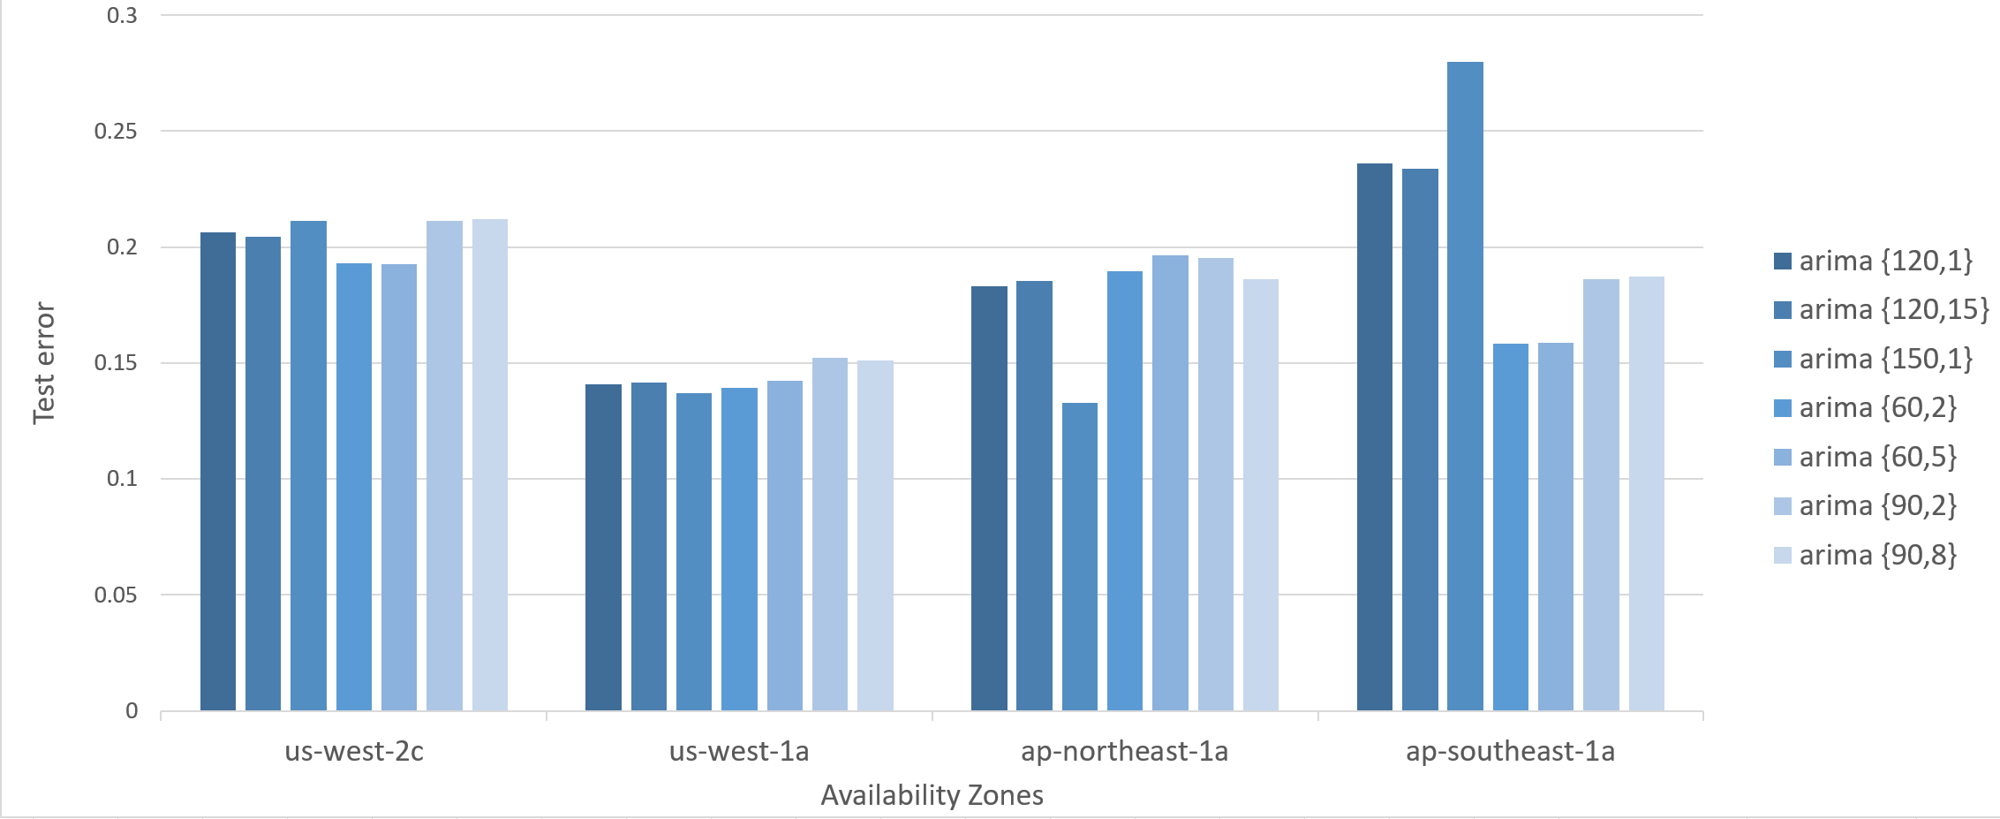
\includegraphics[width=1.2\textwidth]{figures/g2-4M-L.png}\caption{The impact of train data configurations to the overall test error rate of GPU instance.\label{fig:g2-param-diverse}}
\end{figure}
From Figure~\ref{fig:algo-diff-inst}, we observed that the Arima algorithm shows the best performance. As noted earlier, we use various combinations of modeling data period and model use days. To see the effect from the different parameters, we show the test errors of GPU instances for different train data configurations in Figure~\ref{fig:g2-param-diverse}. The left two bars show the test error value of us-west-1a and us-west-2c that show the least impact from the distinct parameters. The right two bars show the test error of ap-northeast-1a and ap-southeast-1a that show the most impact from the paramters. Other availability zones that are not shown in the chart show the pattern in-beetween. In ap-southeast-1a zone, the worst configuration shows 50\% more error rate than the best configuration. Furthermore, the worst configuration in ap-southeast-1a (150, 1) is the best configuration for ap-northeast-1a. We suspect that such diversity was not considered in the previous works that try to predict spot instance price, and they could not eventually find a model to make better prediction. 

\begin{table}
  \begin{tabular}{ |C{2.5cm}||C{2cm}||C{2cm}||C{2cm}||C{2cm}|}
\hline
\small
\textbf{Availability Zones} &\textbf{General}&\textbf{Compute}&\textbf{Memory}&\textbf{Storage}\\\hline
ap-northeast-1a& (60,4)&(60,4)&(60,4)&(120,15)\\
ap-northeast-1c&(60,2)&(60,2)&(120,15)&(120,15)\\
ap-southeast-1a&(150,1)&(150,1)&(150,1)&(150,1)\\
ap-southeast-1b&(150,1)&(60,2)&(150,1)&(150,1)\\
ap-southeast-2a&(60,4)&(60,4)&(150,1)&(150,1)\\
ap-southeast-2b&(60,4)&(60,2)&(150,1)&(120,15)\\
eu-west-1a&(60,4)&(90,8)&(30,2)&(150,1)\\
eu-west-1b&(60,4)&(60,2)&(30,1)&(120,1)\\
eu-west-1c&(60,2)&(60,4)&(30,1)&(150,1)\\
us-east-1a&(50,1)&(150,1)&(30,1)&(60,2)\\
us-east-1c&(150,1)&(150,1)&(30,1)&(150,1)\\
us-east-1d&(60,2)&(150,1)&(30,2)&(150,1)\\
us-east-1e&(60,4)&(150,1)&(30,1)&(60,4)\\
us-west-1a&(60,2)&(150,1)&(30,1)&(120,15)\\
us-west-1b&(60,4)&(150,1)&(30,1)&(120,15)\\
us-west-2a&(60,2)&(150,1)&(150,1)&(150,1)\\
us-west-2b&(60,4)&(150,1)&(30,1)&(150,1)\\
us-west-2c&(60,2)&(60,2)&(60,2)&(150,1)\\\hline
\end{tabular}
\caption{Best Arima model configuration for different instance types in distinct availability zones}
\label{table:best-arima-config}
\end{table}

To check if there is optimal Arima train data configuration, we list the best performing train data parameters in Table~\ref{table:best-arima-config}. From the table, we can see that there is no globally optimal configurations. Contrary to general belief, building a model with train dataset with shorter time window sometimes performs better than longer train dataset. Furthermore, using a model longer period of time ocassionally perform better. From the table, we conclude that predicting spot instace price needs careful consideration in building train dataset, and the configuration needs to be dynamically updated. 


\section{Discussion and Future Work}
With thorough analysis about spot instance price prediction algorithms, we uncover the improved prediction accuracy as well as challenges in making better prediction. Based on the observation, we are going to further improve the algorithm in the following way.  

\textbf{The Good: Spot Price Change Prediction} Most of previous works that tried to predict spot instnace price concluded that the price is random, and applying predictive analysis algorithms does not really help to improve prediction quality~\cite{spot-instance-pricing-analysis,spot-price-han-arima}. In this work, we applied multiple time-series analysis algorithms by carefully designing the period of modeling data and parameters. With extensive evaluation, we could uncover that applying predictive analysis algorithms improves the price prediction accuracy over XY\% comparing to a method that uses only the most recent price~\cite{deep-spot-cloud,not-bid-cloud}.

\textbf{The Challenge: No Globally Optimal Model} Despite of increasing prediction accuracy by applying various techniques, we could not find the globally optimal algorithm and training data specification for different availability zones and distinct instance types. It makes challenging to apply the algorithms for real applications that can be deployed in any environments. 

\textbf{The Promising: Applying Hybrid Models} Even with the diversity of prediction accuracy for different algorithms and train data configuration, it is observed that the train error and test error show high correlation. Pearson product-moment correlation coefficient of train and test error is 0.904 - note that the coefficient has a value from -1.0 to 1.0, and the value of 1.0 means a perfect positive linear correlation, -1.0 means a negative correlation, while 0.0 means no correlation. We currently work on referencing the train error to better choose the algorithms and train data period. We are going to apply the heuristic to an application that utilizes GPU-based AWS EC2 spot instances to execute deep learning tasks in a cost efficient way~\cite{deep-spot-cloud}. 

\textbf{The Benefit: Lower Cost while Using Spot Instances} With the improvement in the prediction accuracy, we expect it will result in the cost gain by cherry-picking few availability zones and instance types with lower prices. We are working on a theoritical model that specifies correlation between the prediction accuracy and the real cost gain. We are also working to utilize the predicted outcome to anticipate instances that are likely to incur unexpected service interruption that is the crucial factor of making users reluctant to use spot instances.  

\section{Conclusion}
Summarize
%\begin{acknowledgement}
%Thanks to ...
%\end{acknowledgement}
\bibliographystyle{spmpsci}
\bibliography{g2-price-modeling}
\end{document}
